\begin{filecontents*}{references.bib}

@misc{goalosSignoffSite,
  author       = {{MontrealAI}},
  title        = {{The Signoff Institution: GoalOS Signoff Pro}},
  year         = {2026},
  howpublished = {\url{https://montrealai.github.io/goalos-signoff-pro/}},
  note         = {Accessed 2026-07-01}
}

@misc{goalosMission001,
  author       = {{MontrealAI}},
  title        = {{Mission 001 Reproducibility Packet: GoalOS Signoff Pro}},
  year         = {2026},
  howpublished = {\url{https://montrealai.github.io/goalos-signoff-pro/mission-001.html}},
  note         = {Accessed 2026-07-01}
}

@misc{goalosNoData,
  author       = {{MontrealAI}},
  title        = {{No user data by design: GoalOS Signoff Pro}},
  year         = {2026},
  howpublished = {\url{https://montrealai.github.io/goalos-signoff-pro/no-user-data.html}},
  note         = {Accessed 2026-07-01}
}

@misc{goalosSettlementLab,
  author       = {{MontrealAI}},
  title        = {{GoalOS Proof-to-Settlement Control Lab}},
  year         = {2026},
  howpublished = {\url{https://montrealai.github.io/goalos-signoff-pro/proof-settlement-lab.html}},
  note         = {Accessed 2026-07-01}
}

@misc{goalosAgialpha,
  author       = {{MontrealAI}},
  title        = {{AGIALPHA is external: GoalOS Signoff Pro}},
  year         = {2026},
  howpublished = {\url{https://montrealai.github.io/goalos-signoff-pro/agialpha.html}},
  note         = {Accessed 2026-07-01}
}

@misc{goalosAgijobmanager,
  author       = {{MontrealAI}},
  title        = {{GoalOS AGIJobManager Ascension}},
  year         = {2026},
  howpublished = {\url{https://montrealai.github.io/goalos-agijobmanager-ascension/}},
  note         = {Accessed 2026-07-01}
}

@misc{goalosRepo,
  author       = {{MontrealAI}},
  title        = {{goalos-signoff-pro GitHub repository}},
  year         = {2026},
  howpublished = {\url{https://github.com/MontrealAI/goalos-signoff-pro}},
  note         = {Accessed 2026-07-01}
}

@misc{goalosReadme,
  author       = {{MontrealAI}},
  title        = {{GoalOS Signoff Pro README}},
  year         = {2026},
  howpublished = {\url{https://raw.githubusercontent.com/MontrealAI/goalos-signoff-pro/main/README.md}},
  note         = {Accessed 2026-07-01}
}

@misc{ethereumOracles,
  author       = {{Ethereum.org}},
  title        = {{Oracles}},
  year         = {2026},
  howpublished = {\url{https://ethereum.org/developers/docs/oracles/}},
  note         = {Accessed 2026-07-01}
}

@misc{buterin2014ethereum,
  author       = {Buterin, Vitalik},
  title        = {{Ethereum: A Next-Generation Smart Contract and Decentralized Application Platform}},
  year         = {2014},
  howpublished = {\url{https://ethereum.org/whitepaper/}}
}

@misc{nakamoto2008bitcoin,
  author       = {Nakamoto, Satoshi},
  title        = {{Bitcoin: A Peer-to-Peer Electronic Cash System}},
  year         = {2008},
  howpublished = {\url{https://bitcoin.org/bitcoin.pdf}}
}

@misc{chainlink2,
  author       = {Breidenbach, Lorenz and Cachin, Christian and Coventry, Ben and Ellis, Steve and Juels, Ari and Koushanfar, Farinaz and Miller, Andrew and Magauran, Brendan and Moroz, Daniel and Nazarov, Sergey and Topliceanu, Alexandru and Tramèr, Florian and Zhang, Fan},
  title        = {{Chainlink 2.0: Next Steps in the Evolution of Decentralized Oracle Networks}},
  year         = {2021},
  howpublished = {\url{https://research.chain.link/whitepaper-v2.pdf}}
}

@misc{w3cProv,
  author       = {{W3C}},
  title        = {{PROV-DM: The PROV Data Model}},
  year         = {2013},
  howpublished = {\url{https://www.w3.org/TR/prov-dm/}}
}

@misc{nistAirmf,
  author       = {{National Institute of Standards and Technology}},
  title        = {{Artificial Intelligence Risk Management Framework (AI RMF 1.0)}},
  year         = {2023},
  howpublished = {\url{https://www.nist.gov/itl/ai-risk-management-framework}}
}

@misc{nistSSDF,
  author       = {{National Institute of Standards and Technology}},
  title        = {{Secure Software Development Framework (SSDF) Version 1.1: NIST SP 800-218}},
  year         = {2022},
  howpublished = {\url{https://csrc.nist.gov/publications/detail/sp/800-218/final}}
}

@misc{slsa,
  author       = {{OpenSSF}},
  title        = {{SLSA: Supply-chain Levels for Software Artifacts}},
  year         = {2026},
  howpublished = {\url{https://slsa.dev/}}
}

@misc{inToto,
  author       = {Torres-Arias, Santiago and Afzali, Hammad and Kuppusamy, Trishank Karthik and Curtmola, Reza and Cappos, Justin},
  title        = {{in-toto: Providing farm-to-table guarantees for bits and bytes}},
  year         = {2019},
  howpublished = {\url{https://in-toto.io/}}
}

@misc{spdx,
  author       = {{Linux Foundation}},
  title        = {{SPDX: Software Package Data Exchange}},
  year         = {2026},
  howpublished = {\url{https://spdx.dev/}}
}

@article{lamport1982byzantine,
  author  = {Lamport, Leslie and Shostak, Robert and Pease, Marshall},
  title   = {{The Byzantine Generals Problem}},
  journal = {ACM Transactions on Programming Languages and Systems},
  volume  = {4},
  number  = {3},
  pages   = {382--401},
  year    = {1982}
}


@misc{nistCyberFramework,
  author       = {{National Institute of Standards and Technology}},
  title        = {{The NIST Cybersecurity Framework 2.0}},
  year         = {2024},
  howpublished = {\url{https://www.nist.gov/cyberframework}},
  note         = {Risk governance and assurance reference}
}

@misc{iso27001,
  author       = {{International Organization for Standardization}},
  title        = {{ISO/IEC 27001 Information security management systems}},
  year         = {2022},
  howpublished = {\url{https://www.iso.org/standard/27001}},
  note         = {Information security management reference}
}

\end{filecontents*}

\documentclass[11pt]{article}

\usepackage[letterpaper,top=0.72in,bottom=0.82in,left=0.74in,right=0.74in,headheight=22pt,includeheadfoot]{geometry}
\usepackage{fontspec}
\defaultfontfeatures{Ligatures=TeX,Scale=MatchLowercase}
\setmainfont{Inter}
\setsansfont{Inter}
\setmonofont{DejaVu Sans Mono}[Scale=0.88]
\usepackage{microtype}
\usepackage{amsmath,amssymb,amsthm,mathtools}
\usepackage{booktabs,tabularx,longtable,array,multirow,makecell}
\usepackage{enumitem}
\usepackage[table]{xcolor}
\usepackage{graphicx}
\usepackage{xurl}
\usepackage{hyperref}
\usepackage[most]{tcolorbox}
\usepackage{tikz}
\usetikzlibrary{arrows.meta,positioning,fit,backgrounds,shapes.geometric,calc,matrix,decorations.pathreplacing}
\usepackage{caption}
\usepackage{subcaption}
\usepackage{listings}
\usepackage{fancyhdr}
\usepackage{titlesec}
\usepackage{lastpage}
\usepackage[backend=biber,style=numeric,sorting=none,natbib=true,maxbibnames=6]{biblatex}
\addbibresource{references.bib}
\usepackage{etoolbox}
\usepackage{needspace}
\usepackage{multicol}
\usepackage{ragged2e}

\hypersetup{
  colorlinks=true,
  linkcolor=NavyInk,
  citecolor=RoyalBlue,
  urlcolor=RoyalBlue,
  pdftitle={Proof Before Settlement: The GoalOS Signoff Pro Standard for Blockchain Credibility},
  pdfauthor={MontrealAI / GoalOS Research Artifact},
  pdfsubject={GoalOS Signoff Pro, blockchain credibility, proof packages, evidence dockets, proof-to-settlement},
  pdfkeywords={GoalOS, Signoff Pro, blockchain, proof package, Evidence Docket, Mission Receipt, settlement, DAO grants, AI agents, trust}
}

% Institutional palette
\definecolor{NavyInk}{HTML}{07182F}
\definecolor{Midnight}{HTML}{0B1220}
\definecolor{RoyalBlue}{HTML}{1D4ED8}
\definecolor{SovereignBlue}{HTML}{0B3D91}
\definecolor{CivicCyan}{HTML}{0F766E}
\definecolor{ImperialPurple}{HTML}{5B21B6}
\definecolor{PrestigeGold}{HTML}{B7791F}
\definecolor{SoftGold}{HTML}{FFF7E6}
\definecolor{SlateText}{HTML}{334155}
\definecolor{MutedText}{HTML}{64748B}
\definecolor{Panel}{HTML}{F8FAFC}
\definecolor{Line}{HTML}{CBD5E1}
\definecolor{Success}{HTML}{166534}
\definecolor{Risk}{HTML}{991B1B}
\definecolor{Amber}{HTML}{92400E}
\definecolor{Mist}{HTML}{EEF6FF}
\definecolor{GoalBlue}{HTML}{0B3D91}
\definecolor{GoalCyan}{HTML}{0F766E}
\definecolor{GoalPurple}{HTML}{6D28D9}
\definecolor{GoalSlate}{HTML}{334155}
\definecolor{GoalLight}{HTML}{F8FAFC}
\definecolor{GoalLine}{HTML}{CBD5E1}
\definecolor{GoalGreen}{HTML}{166534}
\definecolor{GoalRed}{HTML}{991B1B}
\definecolor{GoalAmber}{HTML}{92400E}

\setlist[itemize]{topsep=3pt,itemsep=2pt,leftmargin=1.2em}
\setlist[enumerate]{topsep=3pt,itemsep=2pt,leftmargin=1.45em}
\renewcommand{\arraystretch}{1.18}
\setlength{\parskip}{0.42em}
\setlength{\parindent}{0pt}
\emergencystretch=3em
\setcounter{tocdepth}{2}
\setcounter{secnumdepth}{3}

\pagestyle{fancy}
\fancyhf{}
\lhead{\small\sffamily\color{MutedText} GoalOS Signoff Pro}
\chead{\small\sffamily\color{MutedText} Proof Before Settlement}
\rhead{\small\sffamily\color{MutedText} Institutional Research Paper}
\cfoot{\small\sffamily\color{MutedText} Page \thepage\ of \pageref{LastPage}}
\renewcommand{\headrulewidth}{0.25pt}
\renewcommand{\headrule}{\hbox to\headwidth{\color{Line}\leaders\hrule height \headrulewidth\hfill}}

\titleformat{\section}{\Needspace{8\baselineskip}\Large\bfseries\sffamily\color{NavyInk}}{\thesection}{0.6em}{}
\titleformat{\subsection}{\Needspace{5\baselineskip}\large\bfseries\sffamily\color{SovereignBlue}}{\thesubsection}{0.6em}{}
\titleformat{\subsubsection}{\Needspace{4\baselineskip}\normalsize\bfseries\sffamily\color{SlateText}}{\thesubsubsection}{0.6em}{}
\titlespacing*{\section}{0pt}{1.1em}{0.35em}
\titlespacing*{\subsection}{0pt}{0.8em}{0.25em}

\newtheorem{definition}{Definition}[section]
\newtheorem{proposition}{Proposition}[section]
\newtheorem{theorem}{Theorem}[section]
\newtheorem{corollary}{Corollary}[section]
\newtheorem{assumption}{Assumption}[section]

\tcbset{enhanced,arc=2.5mm,boxrule=0.6pt,left=7pt,right=7pt,top=6pt,bottom=6pt,breakable}
\newtcolorbox{thesisbox}{colback=Mist,colframe=SovereignBlue,title=Core thesis,fonttitle=\bfseries\sffamily}
\newtcolorbox{boundarybox}{colback=SoftGold,colframe=PrestigeGold,title=Claim boundary,fonttitle=\bfseries\sffamily}
\newtcolorbox{standardbox}{colback=CivicCyan!6,colframe=CivicCyan,title=Operational standard,fonttitle=\bfseries\sffamily}
\newtcolorbox{dangerbox}{colback=Risk!5,colframe=Risk,title=Failure mode,fonttitle=\bfseries\sffamily}
\newtcolorbox{prbox}{colback=ImperialPurple!5,colframe=ImperialPurple,title=Public positioning,fonttitle=\bfseries\sffamily}
\newtcolorbox{executivebox}{colback=NavyInk!3,colframe=NavyInk,title=Executive position,fonttitle=\bfseries\sffamily}
\newtcolorbox{mandatebox}{colback=SoftGold,colframe=PrestigeGold,title=Mandate language,fonttitle=\bfseries\sffamily}
\newtcolorbox{evidencebox}{colback=Panel,colframe=Line,title=Evidence note,fonttitle=\bfseries\sffamily}

\lstdefinestyle{goalos}{
  basicstyle=\ttfamily\scriptsize,
  keywordstyle=\bfseries\color{SovereignBlue},
  commentstyle=\itshape\color{MutedText},
  stringstyle=\color{Success},
  showstringspaces=false,
  breaklines=true,
  frame=single,
  rulecolor=\color{Line},
  backgroundcolor=\color{Panel},
  columns=fullflexible,
  numbers=left,
  numberstyle=\tiny\color{MutedText},
  xleftmargin=1.2em,
  framexleftmargin=1.2em
}
\lstset{style=goalos}

\newcommand{\GoalOS}{GoalOS}
\newcommand{\Signoff}{GoalOS Signoff Pro}
\newcommand{\AGIALPHA}{\texttt{\$AGIALPHA}}
\newcommand{\EvidenceDocket}{Evidence Docket}
\newcommand{\ProofBundle}{ProofBundle}
\newcommand{\MissionReceipt}{Mission Receipt}
\newcommand{\NoProof}{\textbf{No Proof. No Trust. No Settlement.}}
\newcommand{\onchain}{on-chain}
\newcommand{\offchain}{off-chain}
\newcommand{\paperVersion}{Elite Institutional Edition v2.0}
\newcommand{\paperDate}{July 1, 2026}

\newcommand{\Rule}{\vspace{0.35em}\noindent{\color{PrestigeGold}\rule{\linewidth}{0.65pt}}\vspace{0.35em}}
\newcommand{\Badge}[1]{\tikz[baseline=(X.base)]\node[fill=NavyInk!5,draw=Line,rounded corners=2pt,inner xsep=5pt,inner ysep=2pt,font=\scriptsize\sffamily\color{SlateText}](X){#1};}
\newcommand{\GoldBadge}[1]{\tikz[baseline=(X.base)]\node[fill=SoftGold,draw=PrestigeGold,rounded corners=2pt,inner xsep=5pt,inner ysep=2pt,font=\scriptsize\sffamily\bfseries\color{Amber}](X){#1};}

\newcommand{\InstitutionalSeal}{%

\begin{tikzpicture}[scale=0.72]
  \draw[PrestigeGold, line width=1pt] (0,0) circle (1.15);
  \draw[PrestigeGold!60, line width=0.5pt] (0,0) circle (0.86);
  \foreach \a in {0,30,...,330}{\draw[PrestigeGold!70] (\a:0.98)--(\a:1.08);}
  \node[font=\sffamily\bfseries\Large, color=PrestigeGold] at (0,0.18) {G};
  \node[font=\sffamily\tiny, color=PrestigeGold] at (0,-0.35) {PROOF};
\end{tikzpicture}%
}

\begin{document}

\begin{titlepage}
\begin{tikzpicture}[remember picture,overlay]
  \fill[Midnight] (current page.south west) rectangle (current page.north east);
  \fill[NavyInk] (current page.south west) rectangle ([xshift=3.15in]current page.north west);
  \fill[SovereignBlue!70!black] ([xshift=3.15in]current page.south west) rectangle ([xshift=3.22in]current page.north west);
  \fill[PrestigeGold] ([xshift=3.22in]current page.south west) rectangle ([xshift=3.25in]current page.north west);
  \draw[PrestigeGold!55, line width=0.4pt] ([xshift=3.55in,yshift=-0.8in]current page.north west) -- ([xshift=7.6in,yshift=-0.8in]current page.north west);
  \draw[PrestigeGold!35, line width=0.4pt] ([xshift=3.55in,yshift=-9.45in]current page.north west) -- ([xshift=7.6in,yshift=-9.45in]current page.north west);
\end{tikzpicture}
\color{white}
\vspace*{0.16in}
\begin{minipage}[t]{0.31\textwidth}
\vspace{0.15in}
\InstitutionalSeal\\[0.35in]
{\sffamily\bfseries\Large GoalOS}\\[-2pt]
{\sffamily\small Signoff Pro}\\[0.45in]
{\small \GoldBadge{INSTITUTIONAL RESEARCH}}\\[0.15in]
{\small \GoldBadge{PUBLIC-ALPHA BOUNDARY}}\\[0.15in]
{\small \GoldBadge{BLOCKCHAIN CREDIBILITY}}\\[0.65in]
{\sffamily\small\color{white!75} Publication control}\\[0.05in]
{\sffamily\small \paperVersion}\\
{\sffamily\small \paperDate}\\[0.65in]
{\sffamily\small\color{white!75} Core standard}\\[0.05in]
{\sffamily\bfseries\large No Proof.}\\[-1pt]
{\sffamily\bfseries\large No Trust.}\\[-1pt]
{\sffamily\bfseries\large No Settlement.}
\end{minipage}\hfill
\begin{minipage}[t]{0.62\textwidth}
\RaggedRight
\vspace{0.42in}
{\sffamily\bfseries\fontsize{34}{36}\selectfont Proof Before}\\[-2pt]
{\sffamily\bfseries\fontsize{34}{36}\selectfont Settlement}\\[0.16in]
{\sffamily\bfseries\fontsize{16}{21}\selectfont The GoalOS Signoff Pro Standard for Blockchain Credibility}\\[0.32in]
{\sffamily\fontsize{13}{18}\selectfont Evidence Dockets, Replayable Receipts, Human Authority, and the Proof Package Mandate}\\[0.52in]
\begin{tcolorbox}[colback=white!6,colframe=PrestigeGold,boxrule=0.8pt,arc=2mm]
{\sffamily\bfseries\large Blockchain proves the transaction. GoalOS proves the work.}\\[3pt]
{\sffamily\normalsize A serious blockchain project should show the proof package before asking for trust, payment, governance authority, or public credibility.}
\end{tcolorbox}
\vfill
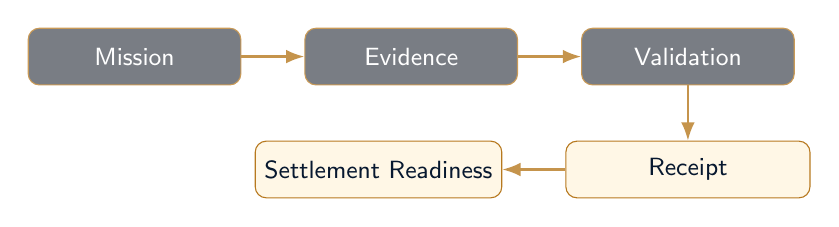
\begin{tikzpicture}[node distance=8mm, every node/.style={font=\sffamily\small}]
  \node[draw=PrestigeGold!75, fill=Midnight!55, rounded corners, minimum width=2.7cm, minimum height=0.72cm, text=white] (m) {Mission};
  \node[draw=PrestigeGold!75, fill=Midnight!55, rounded corners, right=of m, minimum width=2.7cm, minimum height=0.72cm, text=white] (e) {Evidence};
  \node[draw=PrestigeGold!75, fill=Midnight!55, rounded corners, right=of e, minimum width=2.7cm, minimum height=0.72cm, text=white] (v) {Validation};
  \node[draw=PrestigeGold, fill=SoftGold, rounded corners, below=7mm of v, minimum width=3.1cm, minimum height=0.72cm, text=NavyInk] (r) {Receipt};
  \node[draw=PrestigeGold, fill=SoftGold, rounded corners, left=of r, minimum width=3.1cm, minimum height=0.72cm, text=NavyInk] (s) {Settlement Readiness};
  \draw[-{Latex}, thick, color=PrestigeGold!80] (m)--(e);
  \draw[-{Latex}, thick, color=PrestigeGold!80] (e)--(v);
  \draw[-{Latex}, thick, color=PrestigeGold!80] (v)--(r);
  \draw[-{Latex}, thick, color=PrestigeGold!80] (r)--(s);
\end{tikzpicture}\\[0.4in]
{\sffamily\small\color{white!72} Research artifact prepared for institutional communication, technical review, blockchain governance, DAO due diligence, AI-agent settlement design, and public trust standards.}
\end{minipage}
\end{titlepage}

\pagenumbering{roman}
\thispagestyle{empty}
\begin{center}
{\Huge\bfseries\sffamily\color{NavyInk} Executive tear sheet}\\[0.10in]
{\large\sffamily\color{MutedText} The paper in one page}
\end{center}
\Rule
\begin{executivebox}
\textbf{Strategic claim.} Blockchains are excellent at proving that transactions happened. They do not automatically prove that the work behind those transactions was real, complete, reviewed, safe, or worthy of settlement. \Signoff{} supplies the missing credibility layer: mission definition, evidence mapping, replay, validation, risk disclosure, human authority, signed receipt, and optional public commitment.
\end{executivebox}

\begin{center}
\begin{tabularx}{0.96\linewidth}{>{\bfseries\color{NavyInk}}p{0.23\linewidth} X}
\toprule
Institutional message & \textbf{Blockchain proves the transaction. GoalOS proves the work.}\\
Standard & \textbf{No Proof. No Trust. No Settlement.}\\
Primary audience & DAOs, foundations, treasury councils, grant programs, auditors, exchanges, enterprises, AI-agent operators, investors, and protocol governors.\\
Core object & A public-safe proof package: Mission Contract, Evidence Docket, ProofBundle, Replay Log, Validator Report, Risk Ledger, Human Authority Record, Mission Receipt.\\
What v28 adds & The \emph{Blockchain Credibility Standard Lab}: a flagship public demo for proof-before-settlement.\\
What v29 adds & The \emph{Blockchain Proof Mandate and Due Diligence Lab}: a practical demand checklist that asks every project, ``Where is the proof package?''\\
Boundary & Public demos are proof-architecture demonstrations: no wallets, no payments, no custody, no user data, no Mainnet settlement claim.\\
\bottomrule
\end{tabularx}
\end{center}

\begin{mandatebox}
\textbf{Recommended public demand.} Before a blockchain project asks for treasury funds, governance approval, milestone payment, audit closure, AI-agent compensation, RWA credibility, or ecosystem trust, require a GoalOS-style proof package. Not hype. Not dashboard screenshots. Not a vague update. The proof package.
\end{mandatebox}

\newpage
\begin{center}
{\Huge\bfseries\sffamily\color{NavyInk} Publication boundary}\\[0.08in]
{\large\sffamily\color{MutedText} Claim-bounded, public-safe, and adoption-oriented}
\end{center}
\Rule
\begin{boundarybox}
This paper is a research and institutional communication artifact. It is not legal, financial, tax, investment, compliance, cybersecurity certification, external audit, or production-deployment advice. It does not claim live Mainnet settlement, custody, token sale, wallet activation, payment routing, realized AGI, realized ASI, or external factual certification. It specifies a proof architecture and public standard for deciding when off-chain work is mature enough to influence settlement, governance, reputation, or future capability.
\end{boundarybox}

\begin{evidencebox}
\textbf{Grounding.} The live \Signoff{} site presents a proof-to-acceptance console with six gates and public browser-local demos \citep{goalosSignoffSite}. Mission 001 exposes a reproducibility packet containing mission contract, environment, task fixtures, B0--B6 baselines, runner config, proof bundle, replay log, ledgers, verifier report, scoreboard, claims matrix, and replay path \citep{goalosMission001}. The public data posture states no forms, input fields, upload path, wallet connection, payments, cookies, or analytics \citep{goalosNoData}. The proof-to-settlement lab explicitly describes simulation mode: no wallet, no escrow, no payment, no value moved \citep{goalosSettlementLab}.
\end{evidencebox}

\begin{center}
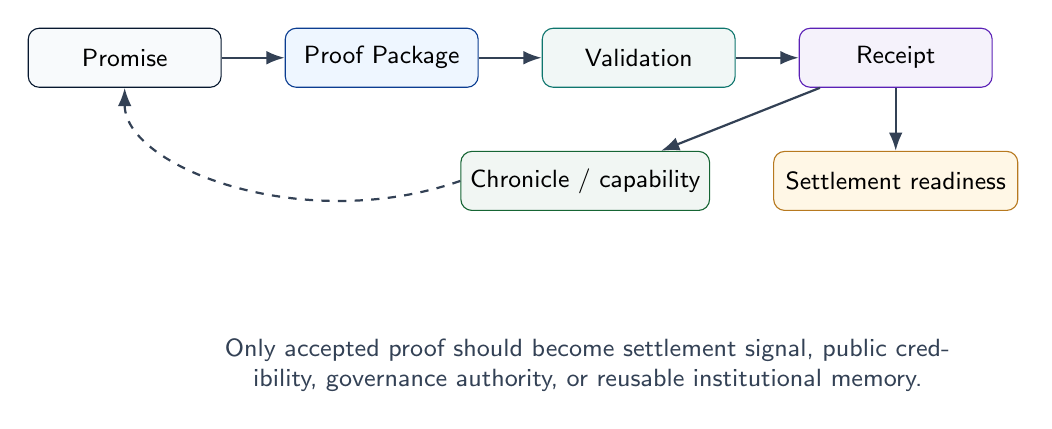
\begin{tikzpicture}[node distance=8mm, every node/.style={font=\sffamily\small}]
\node[draw=NavyInk, fill=Panel, rounded corners, minimum width=2.45cm, minimum height=0.75cm] (a) {Promise};
\node[draw=SovereignBlue, fill=Mist, rounded corners, right=of a, minimum width=2.45cm, minimum height=0.75cm] (b) {Proof Package};
\node[draw=CivicCyan, fill=CivicCyan!6, rounded corners, right=of b, minimum width=2.45cm, minimum height=0.75cm] (c) {Validation};
\node[draw=ImperialPurple, fill=ImperialPurple!6, rounded corners, right=of c, minimum width=2.45cm, minimum height=0.75cm] (d) {Receipt};
\node[draw=PrestigeGold, fill=SoftGold, rounded corners, below=8mm of d, minimum width=3.1cm, minimum height=0.75cm] (e) {Settlement readiness};
\node[draw=Success, fill=Success!6, rounded corners, left=of e, minimum width=3.1cm, minimum height=0.75cm] (f) {Chronicle / capability};
\draw[-{Latex},thick,color=SlateText] (a)--(b);
\draw[-{Latex},thick,color=SlateText] (b)--(c);
\draw[-{Latex},thick,color=SlateText] (c)--(d);
\draw[-{Latex},thick,color=SlateText] (d)--(e);
\draw[-{Latex},thick,color=SlateText] (d)--(f);
\draw[-{Latex},thick,color=SlateText,dashed] (f.west) .. controls +(-2.0,-0.7) and +(0,-1.0) .. (a.south);
\node[below=15mm of f, align=center, text width=0.90\linewidth, font=\sffamily\small\color{SlateText}] {Only accepted proof should become settlement signal, public credibility, governance authority, or reusable institutional memory.};
\end{tikzpicture}
\end{center}

\newpage
\begin{abstract}
Blockchains provide programmable settlement, public state, and tamper-resistant transaction history. They do not, by themselves, prove that the off-chain work behind a transaction was real, complete, independently reviewed, risk-bounded, or worthy of payment. This paper formalizes that missing layer as the \emph{work-verification gap}. We propose \Signoff{} as a proof-to-acceptance and proof-to-settlement architecture for blockchain credibility: a system that converts work claims into mission contracts, evidence dockets, proof bundles, replay logs, validator reports, risk ledgers, human-authority decisions, signed receipts, challenge windows, and optional public anchors. The paper provides a formal object model, lifecycle state machine, acceptance predicate, settlement-safety invariant, threat model, claim-maturity lattice, due-diligence scorecard, and adoption roadmap. It also specifies two flagship public demonstrations: v28, the Blockchain Credibility Standard Lab, and v29, the Blockchain Proof Mandate and Due Diligence Lab. The result is a concise institutional standard: \emph{Blockchain proves the transaction; GoalOS proves the work.} Therefore, for serious blockchain projects: \emph{No Proof. No Trust. No Settlement.}
\end{abstract}

\begin{thesisbox}
\textbf{Contribution.} \Signoff{} is not another blockchain, wallet, oracle, audit badge, or dashboard. It is the proof-and-signoff layer that tells low-trust ecosystems when a claim has matured enough to justify settlement, reputation, governance, or future capability.
\end{thesisbox}

\tableofcontents
\newpage
\pagenumbering{arabic}

\section{Executive summary}

\begin{standardbox}
\begin{center}
{\Large\bfseries Blockchain proves the transaction. GoalOS proves the work.}\\[4pt]
{\large\bfseries No Proof. No Trust. No Settlement.}
\end{center}
\end{standardbox}

Blockchain projects succeed or fail on credibility. The protocol may be transparent, the contract may be deployed, and the transaction may be public, but the work behind the transaction is often still opaque. Was the grant milestone actually completed? Was the audit issue really remediated? Is the upgrade ready? Did the AI agent perform the assigned task? Is the RWA claim supported? Did the vendor deliver what the treasury is about to pay for?

The core answer of this paper is that blockchain credibility needs a proof institution. A proof institution turns off-chain work into structured, inspectable, replayable, signed objects. It is not enough to say that value moved. The ecosystem needs to know why value deserved to move.

\Signoff{} provides that institutional grammar. Its public product language already centers on acceptance: define done, bind evidence, preserve judgment, and issue receipts that executives, reviewers, and systems can independently inspect \citep{goalosSignoffSite}. This paper extends that grammar into a blockchain standard.

The standard is intentionally simple for public adoption:
\begin{center}
\fbox{\begin{minipage}{0.86\linewidth}\centering\sffamily\bfseries\Large Require the proof package before trust, payment, governance, or reputation moves.\end{minipage}}
\end{center}

\subsection*{Why this is strategically important}

Blockchains made settlement programmable. They did not make off-chain work self-verifying. That gap leaves room for milestone ambiguity, grant abuse, audit theater, governance confusion, unauditable AI-agent outputs, and irreversible payments based on insufficient evidence. A GoalOS-style proof package gives every serious stakeholder a practical demand: show the mission, evidence, replay path, validation, risk ledger, human decision, and receipt.

\subsection*{What this paper delivers}

\begin{itemize}
  \item A formal definition of the work-verification gap.
  \item A GoalOS proof object model for blockchain contexts.
  \item A proof-gated lifecycle from mission to settlement readiness.
  \item A settlement-safety invariant: value should not move unless acceptance evidence is mature.
  \item Public demonstration specs for v28 and v29.
  \item Practical adoption templates for DAOs, treasuries, grants, audits, AI-agent settlement, protocol upgrades, and investor due diligence.
\end{itemize}

\begin{executivebox}
\textbf{Bottom line.} Most blockchain projects that ask for public trust should be expected to publish a GoalOS-style proof package. Not because it guarantees success, but because it materially improves credibility, auditability, accountability, and settlement discipline.
\end{executivebox}

\section{Problem: the work-verification gap}

\subsection{Settlement is not acceptance}

Let a blockchain transaction be represented as a state transition
\[
  \delta: (S_t, x, \sigma) \rightarrow S_{t+1},
\]
where $S_t$ is current chain state, $x$ is transaction data, and $\sigma$ is authorization material such as signatures. The chain can verify that $\delta$ is syntactically valid under protocol rules. It can verify signatures, balances, nonces, contract preconditions, gas constraints, and deterministic computation.

But many economically important blockchain decisions depend on a semantic predicate over external work:
\[
  W(M, O, E, R, V, H) \in \{0,1\},
\]
where $M$ is a mission or obligation, $O$ is output, $E$ is evidence, $R$ is replay or reproducibility material, $V$ is validator review, and $H$ is human authority. The chain cannot directly observe $W$ unless a trustworthy representation of $W$ is supplied. This is a broader cousin of the oracle problem. Ethereum's developer documentation describes the oracle problem as the challenge that oracle data must be correct for smart contracts to execute correctly, and that trusting oracle operators can undermine the trustless aspect of smart contracts \citep{ethereumOracles}. The work-verification gap extends that issue from external data to external labor, deliverables, audits, governance claims, and AI-agent outputs.

\begin{definition}[Work-verification gap]
The \emph{work-verification gap} is the distance between (i) an \onchain{} rule that can settle a value-bearing state transition and (ii) the \offchain{} institutional evidence required to know whether the real-world or agentic work motivating that transition has been completed, validated, and accepted.
\end{definition}

\begin{dangerbox}
\textbf{The blind spot.} A DAO can vote to pay a grant; an escrow can release; a token can move; a protocol upgrade can execute. None of these events alone proves that the underlying work was complete, safe, replayable, or accepted by the right authority.
\end{dangerbox}

\subsection{Why informal proof fails at scale}

Informal proof works until projects become high-stakes, multi-party, cross-jurisdictional, or adversarial. At scale, the following failure modes recur:

\begin{enumerate}
  \item \textbf{Milestone ambiguity.} The project cannot determine whether the promised deliverable was achieved because ``done'' was never formalized.
  \item \textbf{Evidence fragmentation.} Relevant evidence is scattered across GitHub, chats, dashboards, PDFs, tweets, audits, and private drives.
  \item \textbf{Output/authority confusion.} A persuasive report is mistaken for accepted work.
  \item \textbf{Replay failure.} Reviewers cannot reproduce or inspect the claimed result.
  \item \textbf{Reviewer opacity.} It is unclear who validated what, under which criteria, and with what conflicts.
  \item \textbf{Risk laundering.} Known caveats disappear as the claim moves from technical review to public communication.
  \item \textbf{Settlement irreversibility.} Funds, reputation, governance weight, or public claims move before evidence is mature.
  \item \textbf{Memory contamination.} Unsupported work influences future missions, model routing, or protocol decisions.
\end{enumerate}

\subsection{Blockchain projects are especially exposed}

Blockchain projects often combine low-trust coordination with irreversible consequences. Contributors may not know each other. DAO delegates may review complex claims under time pressure. Grant programs need to fund work without creating rent-seeking. Protocol upgrades can affect users who did not participate in the decision. Oracles and bridges depend on external assumptions. AI agents may produce outputs that look plausible but are difficult to verify. In this environment, trust should not depend on charisma, marketing, dashboard aesthetics, or social momentum. It should depend on a proof package.

\section{Design thesis}

\begin{prbox}
\textbf{Public thesis.} Most serious blockchain projects should be expected to publish a GoalOS-style proof package before asking for public trust, treasury funds, governance approval, ecosystem credibility, or settlement. The simplest demand is: \emph{Where is the proof package?}
\end{prbox}

The design thesis is that blockchain credibility requires three layers:

\begin{enumerate}
  \item \textbf{Computational settlement.} The chain executes deterministic rules and preserves public state.
  \item \textbf{Proof institution.} GoalOS structures the \offchain{} work into inspectable proof packages.
  \item \textbf{Authority and memory.} Accepted proof becomes a receipt, an optional anchor, and a controlled source of future capability or reputation.
\end{enumerate}

\begin{figure}[h]
\centering
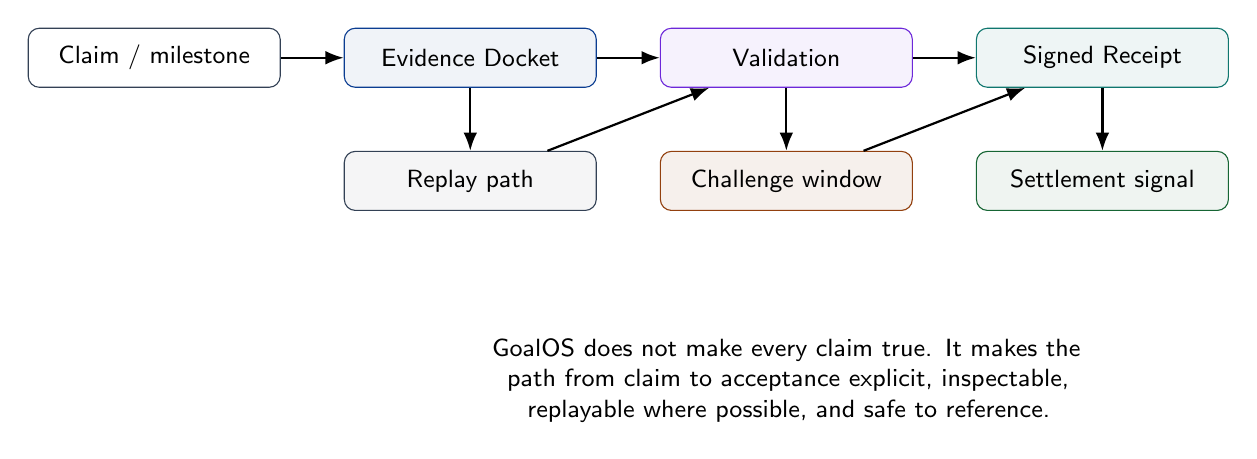
\begin{tikzpicture}[node distance=8mm, every node/.style={font=\sffamily\small}]
\node[draw=GoalSlate, rounded corners, fill=white, minimum width=3.2cm, minimum height=0.75cm] (claim) {Claim / milestone};
\node[draw=GoalBlue, rounded corners, fill=GoalBlue!6, right=of claim, minimum width=3.2cm, minimum height=0.75cm] (docket) {Evidence Docket};
\node[draw=GoalPurple, rounded corners, fill=GoalPurple!6, right=of docket, minimum width=3.2cm, minimum height=0.75cm] (review) {Validation};
\node[draw=GoalCyan, rounded corners, fill=GoalCyan!7, right=of review, minimum width=3.2cm, minimum height=0.75cm] (receipt) {Signed Receipt};
\node[draw=GoalGreen, rounded corners, fill=GoalGreen!7, below=8mm of receipt, minimum width=3.2cm, minimum height=0.75cm] (settle) {Settlement signal};
\node[draw=GoalAmber, rounded corners, fill=GoalAmber!8, below=8mm of review, minimum width=3.2cm, minimum height=0.75cm] (challenge) {Challenge window};
\node[draw=GoalSlate, rounded corners, fill=GoalSlate!5, below=8mm of docket, minimum width=3.2cm, minimum height=0.75cm] (replay) {Replay path};
\draw[-{Latex}, thick] (claim)--(docket);
\draw[-{Latex}, thick] (docket)--(review);
\draw[-{Latex}, thick] (review)--(receipt);
\draw[-{Latex}, thick] (receipt)--(settle);
\draw[-{Latex}, thick] (docket)--(replay);
\draw[-{Latex}, thick] (replay)--(review);
\draw[-{Latex}, thick] (review)--(challenge);
\draw[-{Latex}, thick] (challenge)--(receipt);
\node[align=center, below=15mm of challenge, text width=0.86\textwidth] {GoalOS does not make every claim true. It makes the path from claim to acceptance explicit, inspectable, replayable where possible, and safe to reference.};
\end{tikzpicture}
\caption{GoalOS as the missing institutional layer between claims and settlement.}
\label{fig:goalos-layer}
\end{figure}

\subsection{Non-goals}

The architecture is deliberately bounded. It is not a claim that public demos already perform live settlement. It is not a wallet, broker, exchange, custodian, token-sale mechanism, legal certification engine, or source of investment advice. The live Signoff Pro site states a no-data public posture, and its \AGIALPHA{} boundary page says the token is external and not sold, issued, brokered, custodied, distributed, redeemed, staked, or made available by GoalOS, MontrealAI, or QuebecAI \citep{goalosNoData,goalosAgialpha}. The AGIJobManager Ascension public site similarly states that public pages are read-only and do not connect wallets, approve tokens, broadcast transactions, authorize funds, certify external factual correctness, or grant production authority \citep{goalosAgijobmanager}.

\begin{boundarybox}
\textbf{Research boundary.} This paper specifies a proof architecture and demonstration standard. It does not claim live economic activation. The strongest current claim is: GoalOS demonstrates a public-alpha proof-to-acceptance architecture and can be extended into a proof-to-settlement standard when external review, challenge windows, anchoring, and production authorization are independently established.
\end{boundarybox}

\section{Related work}

\subsection{Blockchains and programmable settlement}

Bitcoin introduced a peer-to-peer electronic cash system using proof-of-work consensus to order transactions without a central intermediary \citep{nakamoto2008bitcoin}. Ethereum generalized blockchain execution through smart contracts and decentralized applications \citep{buterin2014ethereum}. These systems made settlement programmable, but they did not eliminate the need to reason about external facts and work.

\subsection{Oracles and hybrid smart contracts}

Oracles address the fact that smart contracts require access to external data and systems. Ethereum documentation frames the oracle problem as the need for oracle data to be correct, available, and incentive-compatible \citep{ethereumOracles}. Chainlink 2.0 expands the oracle idea toward decentralized oracle networks that provide external connectivity and off-chain computation for hybrid smart contracts \citep{chainlink2}. GoalOS is complementary: it does not merely provide data to a contract; it structures the evidence, validation, replay, risk, and human acceptance surrounding work.

\subsection{Provenance, auditability, and reproducibility}

W3C PROV supplies a data model for representing entities, activities, agents, and their provenance relationships \citep{w3cProv}. Modern software supply-chain frameworks such as SLSA, in-toto, and SPDX provide lessons for artifact integrity, attestation, and dependency transparency \citep{slsa,inToto,spdx}. NIST's AI Risk Management Framework emphasizes governance, mapping, measuring, and managing AI risk \citep{nistAirmf}. NIST's Secure Software Development Framework captures practices for reducing software vulnerabilities and improving traceability \citep{nistSSDF}. GoalOS imports this general discipline into blockchain and agentic work: not just code provenance, but mission provenance; not just dependency transparency, but claim transparency; not just audit logs, but acceptance receipts.

\subsection{DAOs and governance}

DAOs attempt to coordinate decisions and resources through tokenized or cryptographic governance. Their weakness is often not the absence of a vote, but the absence of a high-quality evidentiary object before a vote. A GoalOS proof package can act as the evidence object that makes DAO votes, grants, and treasury disbursements more credible.

\section{The GoalOS proof object model}

This section defines the core artifacts. The terminology is designed to be precise enough for engineers and obvious enough for non-technical stakeholders.

\begin{definition}[Mission Contract]
A \emph{Mission Contract} is a bounded specification of work. It defines objective, scope, success criteria, failure criteria, constraints, risk class, allowed actions, denied actions, evidence requirements, reviewer roles, budget limits, challenge window, and done condition.
\end{definition}

\begin{definition}[Evidence Docket]
An \emph{Evidence Docket} is a structured proof room that maps claims to evidence, replay material, provenance, validator notes, risk status, acceptance decisions, and public/private boundaries.
\end{definition}

\begin{definition}[ProofBundle]
A \emph{ProofBundle} is a compact cryptographic and procedural summary of a work execution: trace roots, output hashes, input commitments, environment commitments, policy decisions, cost and latency records, signatures, and any replay material required by the mission.
\end{definition}

\begin{definition}[Mission Receipt]
A \emph{Mission Receipt} is an immutable acceptance record. It references the mission, evidence docket, validation state, human decision, timestamp, signature metadata, and optional on-chain anchor. It is the settlement-adjacent object, not the raw output.
\end{definition}

\begin{definition}[Chronicle]
A \emph{Chronicle} is controlled institutional memory. Only accepted proof may become memory, reusable capability, reputation, or future routing authority. Rejected, challenged, or unsupported outputs may become warnings but not authority.
\end{definition}

\begin{longtable}{p{0.20\textwidth} p{0.28\textwidth} p{0.24\textwidth} p{0.18\textwidth}}
\caption{GoalOS proof object taxonomy.}\label{tab:taxonomy}\\
\toprule
\textbf{Object} & \textbf{Question answered} & \textbf{Typical content} & \textbf{Settlement role}\\
\midrule
\endfirsthead
\toprule
\textbf{Object} & \textbf{Question answered} & \textbf{Typical content} & \textbf{Settlement role}\\
\midrule
\endhead
Mission Contract & What exactly was promised? & Objective, criteria, scope, risk, budget, allowed actions & Defines settlement conditions \\
Evidence Docket & What proof exists? & Claims, artifacts, mappings, provenance, caveats & Enables review \\
ProofBundle & What can be cryptographically and procedurally checked? & Hashes, trace roots, signatures, environment commitments & Enables replay/anchoring \\
Replay Log & Can the result be reproduced or inspected? & Deterministic stages, commands, validators, outputs & Blocks unsupported claims \\
Validator Report & Who reviewed what? & Verdicts, disagreements, quorum, challenge outcomes & Provides confidence and accountability \\
Risk Ledger & What could still go wrong? & Safety events, policy issues, residual risk, rollback status & Controls release class \\
Human Authority Record & Who accepted it? & Signoff identity, role, timestamp, decision reason & Preserves authority boundary \\
Mission Receipt & What exact object can systems reference? & Acceptance hash, evidence hash, decision state, signature & Settlement-adjacent receipt \\
Anchor & What public commitment exists? & Receipt hash, CID, timestamp, revocation state & Tamper-evident reference \\
Chronicle Entry & What may influence future work? & Accepted lessons, warnings, capability updates & Controls compounding \\
\bottomrule
\end{longtable}

\section{Formal architecture}

\subsection{Participants}

Let the system include the following actors:
\[
  \mathcal{A}=\{q,w,v,h,t,c\},
\]
where $q$ is a requester, $w$ is a worker or agent, $v$ is a validator set, $h$ is a human authority, $t$ is a treasury or settlement system, and $c$ is a chain or public commitment layer.

Actors are not assumed to trust each other. The system aims to make trust decisions explicit through artifacts, signatures, quorum rules, challenge windows, and public commitments.

\subsection{State machine}

A mission is represented by a state variable over proof-gated lifecycle states:
\[
\begin{aligned}
  s \in \{&\textsf{draft},\ \textsf{commissioned},\ \textsf{executed},\ \textsf{docketed},\ 
  \textsf{review},\ \textsf{challenged},\\
  &\textsf{accepted},\ \textsf{receipted},\ \textsf{settlement\_ready},\ 
  \textsf{chronicled},\ \textsf{rejected}\}.
\end{aligned}
\]

\begin{figure}[h]
\centering
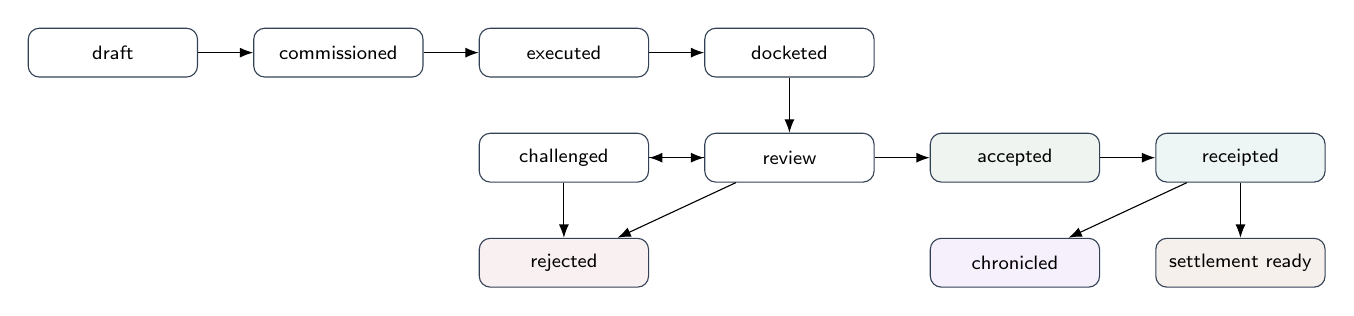
\begin{tikzpicture}[node distance=7mm, every node/.style={font=\sffamily\scriptsize}]
\tikzstyle{state}=[draw=GoalSlate, rounded corners, fill=white, minimum width=2.15cm, minimum height=0.62cm]
\node[state] (draft) {draft};
\node[state, right=of draft] (comm) {commissioned};
\node[state, right=of comm] (exec) {executed};
\node[state, right=of exec] (docket) {docketed};
\node[state, below=of docket] (review) {review};
\node[state, left=of review] (challenge) {challenged};
\node[state, right=of review, fill=GoalGreen!7] (accept) {accepted};
\node[state, right=of accept, fill=GoalCyan!7] (receipt) {receipted};
\node[state, below=of receipt, fill=GoalAmber!8] (settle) {settlement ready};
\node[state, left=of settle, fill=GoalPurple!7] (chron) {chronicled};
\node[state, below=of challenge, fill=GoalRed!6] (reject) {rejected};
\draw[-{Latex}] (draft)--(comm);
\draw[-{Latex}] (comm)--(exec);
\draw[-{Latex}] (exec)--(docket);
\draw[-{Latex}] (docket)--(review);
\draw[-{Latex}] (review)--(challenge);
\draw[-{Latex}] (challenge)--(review);
\draw[-{Latex}] (review)--(accept);
\draw[-{Latex}] (accept)--(receipt);
\draw[-{Latex}] (receipt)--(settle);
\draw[-{Latex}] (receipt)--(chron);
\draw[-{Latex}] (review)--(reject);
\draw[-{Latex}] (challenge)--(reject);
\end{tikzpicture}
\caption{Mission lifecycle as a proof-gated state machine.}
\label{fig:state-machine}
\end{figure}

\subsection{Acceptance predicate}

Let $M$ be a mission contract, $D$ an evidence docket, $P$ a proof bundle, $L$ a replay log, $R$ a risk ledger, $V$ a validator report, $H$ a human-authority record, and $\Gamma$ a policy context. We define the acceptance predicate:
\[
\mathsf{Accept}(M,D,P,L,R,V,H;\Gamma)=1
\]
iff all required gates are satisfied:
\begin{align*}
\mathsf{Complete}(D,M)&=1,\\
\mathsf{MappedClaims}(D,M)&=1,\\
\mathsf{Replayable}(P,L,M)&=1,\\
\mathsf{ValidatorQuorum}(V,\Gamma)&=1,\\
\mathsf{RiskWithinBoundary}(R,M,\Gamma)&=1,\\
\mathsf{ChallengeCleared}(D,V,\Gamma)&=1,\\
\mathsf{HumanAuthority}(H,M,\Gamma)&=1.
\end{align*}

If any gate fails, the mission may remain useful as a draft, warning, or partial artifact, but it does not become settlement-ready.

\begin{theorem}[Settlement safety invariant]
Assume the acceptance predicate above is a necessary precondition for every settlement transition. Then no reachable settlement-ready state exists for a mission that lacks complete evidence, mapped claims, replay material required by policy, validator quorum, risk clearance, challenge clearance, or required human authority.
\end{theorem}

\begin{proof}
By construction, the transition relation into $\textsf{settlement\_ready}$ contains $\mathsf{Accept}$ as a necessary precondition. $\mathsf{Accept}$ is a conjunction of the seven gate predicates above. If any gate fails, the conjunction evaluates to $0$, so the transition is disabled. Therefore no execution trace can reach $\textsf{settlement\_ready}$ unless all required gates hold. This is a protocol safety result, not an empirical claim that the evidence is externally true.
\end{proof}

\subsection{Claim maturity lattice}

Claims should not be binary. They mature through proof states. The path can be read in two lines:
\[
\begin{array}{c}
\textsf{unsupported} \prec \textsf{docketed} \prec \textsf{mapped} \prec \textsf{replayed} \prec \textsf{validated} \\
\prec\ \textsf{challenge\_cleared} \prec \textsf{accepted} \prec \textsf{receipted} \prec \textsf{settlement\_ready} \prec \textsf{reusable}.
\end{array}
\]

\begin{figure}[h]
\centering
\resizebox{0.96\textwidth}{!}{%
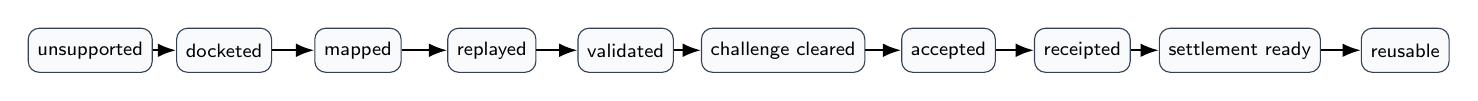
\begin{tikzpicture}[node distance=5mm, every node/.style={font=\sffamily\scriptsize}]
\foreach \name/\label/\x in {u/unsupported/0,d/docketed/1.7,m/mapped/3.4,r/replayed/5.1,v/validated/6.8,c/challenge cleared/8.8,a/accepted/10.9,rec/receipted/12.6,s/settlement ready/14.6,re/reusable/16.7}{
  \node[draw=GoalSlate, rounded corners, fill=GoalLight, minimum height=0.56cm] (\name) at (\x,0) {\label};
}
\draw[-{Latex}, thick] (u)--(d);
\draw[-{Latex}, thick] (d)--(m);
\draw[-{Latex}, thick] (m)--(r);
\draw[-{Latex}, thick] (r)--(v);
\draw[-{Latex}, thick] (v)--(c);
\draw[-{Latex}, thick] (c)--(a);
\draw[-{Latex}, thick] (a)--(rec);
\draw[-{Latex}, thick] (rec)--(s);
\draw[-{Latex}, thick] (s)--(re);
\end{tikzpicture}%
}
\caption{A claim-maturity lattice prevents premature settlement and premature memory.}
\label{fig:lattice}
\end{figure}

\subsection{Proof debt}

We define proof debt as the residual deficit between required proof and available proof. Let $G=\{g_1,\dots,g_n\}$ be required gates with weights $\omega_i$, and let $z_i\in\{0,1\}$ indicate whether gate $g_i$ is satisfied. Proof debt is
\[
  \mathsf{Debt}(M,D,P)=\sum_{i=1}^{n}\omega_i(1-z_i).
\]
Settlement readiness requires $\mathsf{Debt}=0$ for mandatory gates and $\mathsf{Debt}\leq\tau$ for optional or risk-adjusted gates. The public interface can express this in plain language: what is still missing before anyone should trust the claim?

\subsection{Economic control interface}

Let $Q(P)$ be proof quality, $U(M)$ mission utility, $K(M)$ risk class, $C(P)$ cost, and $D(P)$ proof debt. A synthetic proof-work-unit score can be represented as
\[
  \alpha\mathrm{WU}(M,P)=\lambda_1 U(M)Q(P)-\lambda_2 D(P)-\lambda_3 K(M)-\lambda_4 C(P),
\]
where $\lambda_i\geq0$ are policy weights. This score should not be confused with live token settlement. It is an internal control signal that can inform budgets, validator intensity, challenge windows, and readiness decisions.

\section{Protocol: Proof-to-Settlement}

\subsection{Plain-English protocol}

\begin{enumerate}
  \item \textbf{Request.} A requester states the objective and risk class.
  \item \textbf{Mission.} GoalOS converts the objective into a Mission Contract.
  \item \textbf{Work.} Workers or agents execute within bounded allowed actions.
  \item \textbf{Proof.} Outputs are packaged with evidence, traces, hashes, costs, and risks.
  \item \textbf{Docket.} Claims are mapped to evidence and caveats.
  \item \textbf{Replay.} Reviewers attempt reproduction or inspect replay commitments.
  \item \textbf{Validate.} Validators render verdicts under a quorum rule.
  \item \textbf{Challenge.} The system opens a challenge window for contested claims.
  \item \textbf{Authorize.} Human authority accepts, rejects, or holds the mission.
  \item \textbf{Receipt.} A signed receipt is issued for accepted work.
  \item \textbf{Anchor.} Optional hash anchoring creates tamper-evident public reference.
  \item \textbf{Settle.} Treasury, escrow, governance, reputation, or routing may act on the receipt.
  \item \textbf{Chronicle.} Accepted proof becomes controlled memory or reusable capability.
\end{enumerate}

\subsection{Protocol sketch}

\begin{lstlisting}[language=Python, caption={GoalOS proof-to-settlement protocol sketch.}]
def proof_to_settlement(request, policy):
    mission = compile_mission_contract(request, policy)
    work = execute_bounded_work(mission)
    proof = build_proof_bundle(work, mission)
    docket = map_claims_to_evidence(mission, work, proof)
    replay = run_or_record_replay(docket, mission)
    risk = produce_risk_ledger(docket, replay, policy)
    validation = collect_validator_report(docket, replay, risk, policy)
    challenge = run_challenge_window(docket, validation, policy)
    authority = collect_human_authority(mission, docket, validation, risk)

    if accept(mission, docket, proof, replay, risk, validation, challenge, authority):
        receipt = issue_signed_receipt(mission, docket, validation, authority)
        anchor = maybe_anchor_receipt_hash(receipt, policy)
        return settlement_ready(receipt, anchor)

    return reject_or_hold(mission, docket, validation, risk, challenge)
\end{lstlisting}

\subsection{On-chain and off-chain split}

A credible implementation should put rich evidence \offchain{} and compact commitments \onchain{}.

\begin{longtable}{p{0.30\textwidth} p{0.30\textwidth} p{0.30\textwidth}}
\caption{Recommended off-chain/on-chain split.}\label{tab:split}\\
\toprule
\textbf{Layer} & \textbf{Store off-chain} & \textbf{Commit on-chain}\\
\midrule
\endfirsthead
\toprule
\textbf{Layer} & \textbf{Store off-chain} & \textbf{Commit on-chain}\\
\midrule
\endhead
Mission & Full contract, criteria, risk class & Mission hash, version, policy root \\
Evidence & Files, reviews, logs, redactions & Docket hash, content identifier, timestamp \\
Replay & Full replay logs and deterministic artifacts & Replay root, environment root \\
Validation & Validator notes, conflicts, evidence mapping & Validator report hash, quorum flag \\
Authority & Human decision rationale & Receipt hash, signer identity commitment \\
Settlement & Treasury context, payment authorization docs & Settlement-ready receipt hash, revocation status \\
Chronicle & Lessons, reusable capability package & Chronicle entry hash, capability version hash \\
\bottomrule
\end{longtable}

\begin{proposition}[Anchoring is not truth]
A receipt hash anchored on-chain makes a particular receipt tamper-evident and time-referenced. It does not by itself prove that the underlying work is true, complete, safe, or legally sufficient.
\end{proposition}

\begin{proof}
A hash commitment binds to bytes, not to external semantic truth. Truth claims require evidence, replay, validation, challenge, risk review, and authority. Anchoring strengthens integrity of the accepted record; it does not replace validation.
\end{proof}

\section{Blockchain applications}

\subsection{DAO grants}

DAO grant programs are the cleanest early use case. A grant proposal can be converted into a Mission Contract. Each milestone produces an Evidence Docket. Reviewers validate outputs. The DAO or grant committee accepts, holds, or rejects the milestone. A Mission Receipt becomes the object referenced by treasury action.

\begin{standardbox}
\textbf{DAO grant rule.} No milestone payout without a proof package: mission, evidence, replay or inspection route, validator review, risk ledger, human or committee signoff, and receipt.
\end{standardbox}

\subsection{Audit remediation}

Audit remediation often fails because teams claim issues are fixed but reviewers lack a structured packet connecting findings to patches, tests, replay logs, and residual risk. GoalOS can map each finding to a remediation mission, proof bundle, test evidence, reviewer verdict, and final authority.

\subsection{Protocol upgrades}

Protocol upgrades should be gated by evidence, simulation, rollback analysis, challenge windows, and human/governance authority. GoalOS can provide a release-readiness docket that distinguishes a persuasive upgrade narrative from an accepted upgrade proof.

\subsection{AI-agent settlement}

Agentic systems increase the urgency of proof-gated settlement. If agents can generate work, request funds, trigger workflows, or influence governance, then output-only acceptance is unsafe. The rule becomes: no ProofBundle, no agent settlement signal; no replay, no propagation; no rollback, no release.

\subsection{Real-world asset and oracle-adjacent workflows}

For RWA and oracle-adjacent systems, GoalOS can structure the evidence around provenance, attestations, redactions, challenge windows, and claim boundaries. It should not claim to solve every external truth problem. It should make the truth claim accountable and inspectable before settlement depends on it.

\section{v28 and v29: public demonstration architecture}

\subsection{v28: Blockchain Credibility Standard Lab}

The v28 lab should be the public flagship for blockchain audiences. Its purpose is to make the standard unforgettable:

\begin{center}
{\Large\bfseries Blockchain proves the transaction. GoalOS proves the work.}\\[2pt]
{\large\bfseries Do not just move value. Prove it was earned.}
\end{center}

\subsubsection*{Required v28 sections}

\begin{enumerate}
  \item \textbf{The trust gap.} Show why transaction transparency is not work verification.
  \item \textbf{The proof package.} Show mission, evidence, replay, validation, risk, human signoff, receipt, and anchor.
  \item \textbf{Use-case switcher.} DAO grant, audit remediation, protocol upgrade, AI-agent work, RWA claim, partnership milestone.
  \item \textbf{Settlement readiness console.} Show why output-only claims fail and proof-cleared claims pass.
  \item \textbf{Boundary panel.} State no wallet, no payment, no Mainnet transaction, no legal/financial advice, zero value moved.
  \item \textbf{Downloadable artifacts.} Provide public-safe JSON bundles and a public proof-dashboard schema.
\end{enumerate}

\subsection{v29: Blockchain Proof Mandate and Due Diligence Lab}

The v29 lab should convert v28's thesis into a user action: require the proof package.

\begin{center}
{\Large\bfseries Where is the proof package?}\\[2pt]
{\large\bfseries No proof package, no serious trust.}
\end{center}

\subsubsection*{Required v29 sections}

\begin{enumerate}
  \item \textbf{Stakeholder selector.} User, DAO delegate, grant committee, auditor, investor, partner, enterprise buyer, exchange, AI-agent operator.
  \item \textbf{Proof request card.} A one-screen checklist for asking a blockchain project to prove its claim.
  \item \textbf{Due diligence scorecard.} Score evidence completeness, replayability, validator independence, risk disclosure, authority, and receipt integrity.
  \item \textbf{Mandate templates.} DAO policy, grant RFP clause, treasury payment rule, exchange review clause, partner procurement clause.
  \item \textbf{Decision tree.} Accept, hold, challenge, reject, or request missing evidence.
  \item \textbf{Public copy bank.} Social, README, docs, and governance wording.
\end{enumerate}

\subsection{v28/v29 as a communication stack}

\begin{figure}[h]
\centering
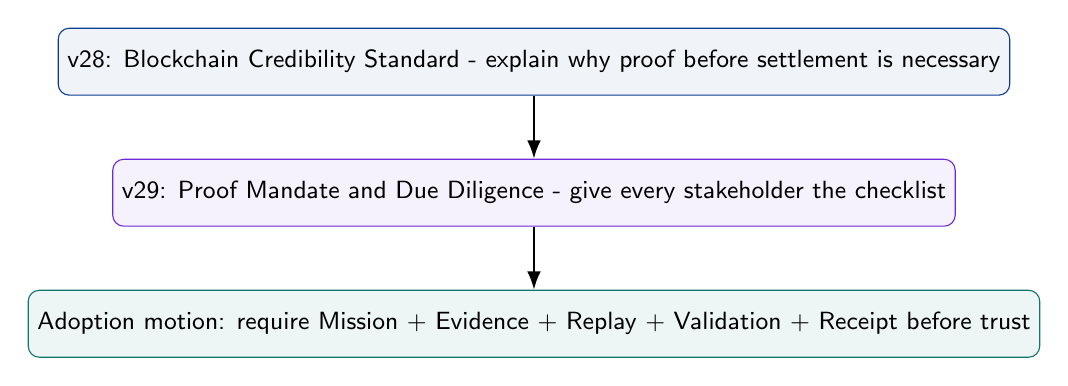
\begin{tikzpicture}[node distance=8mm, every node/.style={font=\sffamily\small}]
\node[draw=GoalBlue, fill=GoalBlue!6, rounded corners, minimum width=10.5cm, minimum height=0.85cm] (v28) {v28: Blockchain Credibility Standard - explain why proof before settlement is necessary};
\node[draw=GoalPurple, fill=GoalPurple!6, rounded corners, below=of v28, minimum width=10.5cm, minimum height=0.85cm] (v29) {v29: Proof Mandate and Due Diligence - give every stakeholder the checklist};
\node[draw=GoalCyan, fill=GoalCyan!7, rounded corners, below=of v29, minimum width=10.5cm, minimum height=0.85cm] (adopt) {Adoption motion: require Mission + Evidence + Replay + Validation + Receipt before trust};
\draw[-{Latex}, thick] (v28)--(v29);
\draw[-{Latex}, thick] (v29)--(adopt);
\end{tikzpicture}
\caption{v28 makes the idea obvious; v29 makes the demand operational.}
\label{fig:v28v29}
\end{figure}

\section{Threat model}

\subsection{Adversaries}

The system should assume adversarial or misaligned behavior from workers, requesters, validators, governance voters, data providers, and external systems.

\begin{longtable}{p{0.20\textwidth} p{0.30\textwidth} p{0.36\textwidth}}
\caption{Threat model and GoalOS controls.}\label{tab:threats}\\
\toprule
\textbf{Threat} & \textbf{Attack} & \textbf{Control}\\
\midrule
\endfirsthead
\toprule
\textbf{Threat} & \textbf{Attack} & \textbf{Control}\\
\midrule
\endhead
Output laundering & Persuasive narrative without proof & Mandatory docket and claim-evidence mapping \\
Evidence stuffing & Large irrelevant artifact dump & Criteria mapping, reviewer burden score, proof debt \\
Replay gap & Hashes exist but no reproduction route & Replay gate and independent replay status \\
Validator capture & Colluding or low-quality reviewers & Quorum rules, conflict disclosure, challenge windows \\
Risk hiding & Known caveats omitted from public claim & Risk ledger and claim-boundary firewall \\
Premature settlement & Funds move before review completes & Settlement safety invariant \\
Privacy leakage & Sensitive execution details exposed & Redaction maps and public/private proof boundary \\
Governance theater & Vote proceeds without evidence & Proof package mandate and due-diligence scorecard \\
Memory contamination & Failed claims influence future work & Chronicle rule: accepted proof only \\
Token confusion & Demo mistaken for live financial rail & Boundary pages, no-wallet demos, synthetic signals only \\
\bottomrule
\end{longtable}

\subsection{Safety properties}

A production-grade proof-to-settlement system should target the following properties:

\begin{itemize}
  \item \textbf{Integrity.} Receipts bind to exact evidence and decision state.
  \item \textbf{Replayability.} Required claims expose reproduction or inspection routes.
  \item \textbf{Accountability.} Reviewers, validators, and authorities are recorded.
  \item \textbf{Minimal disclosure.} Public proof commitments do not leak private execution details.
  \item \textbf{Revocability.} Receipts can be superseded or revoked when evidence fails.
  \item \textbf{Challengeability.} Claims can be contested before settlement or propagation.
  \item \textbf{Human boundary.} High-risk work preserves explicit human authority.
  \item \textbf{No silent compounding.} Only accepted proof influences future work.
\end{itemize}

\section{Implementation blueprint}

\subsection{Minimal viable public standard}

A project can start without live wallets or settlement. The public standard requires only:

\begin{enumerate}
  \item Mission Contract template.
  \item Evidence Docket template.
  \item Claims Matrix.
  \item Replay or inspection checklist.
  \item Validator report.
  \item Risk ledger.
  \item Human signoff record.
  \item Signed Mission Receipt.
  \item Optional hash anchor.
  \item Public proof dashboard.
\end{enumerate}

\subsection{GitHub-native implementation}

A practical route for public projects is GitHub-native:

\begin{itemize}
  \item Store public-safe mission and proof artifacts in version control.
  \item Generate proof pages with GitHub Actions.
  \item Publish static proof dashboards to GitHub Pages.
  \item Produce machine-readable JSON receipts.
  \item Gate settlement-related PRs on validation checks.
  \item Use branch protection for proof artifacts.
\end{itemize}

The current GoalOS Signoff Pro repository is already positioned as a public demo layer for acceptance, evidence review, signed receipts, optional verified receipts, browser-local demos, sample artifacts, and GitHub Actions generation \citep{goalosRepo,goalosReadme}.

\subsection{Maturity levels}

\begin{longtable}{p{0.12\textwidth} p{0.26\textwidth} p{0.32\textwidth} p{0.20\textwidth}}
\caption{GoalOS blockchain credibility maturity model.}\label{tab:maturity}\\
\toprule
\textbf{Level} & \textbf{Name} & \textbf{Capability} & \textbf{Public claim}\\
\midrule
\endfirsthead
\toprule
\textbf{Level} & \textbf{Name} & \textbf{Capability} & \textbf{Public claim}\\
\midrule
\endhead
0 & Narrative & Project describes work with no evidence package & Marketing only \\
1 & Docketed & Claims mapped to public-safe evidence & Reviewable claim \\
2 & Replayable & Replay or inspection path exists & Reproducible or inspectable \\
3 & Validated & Independent validator report attached & Validator-reviewed \\
4 & Receipted & Human authority signs acceptance receipt & Institutionally accepted \\
5 & Anchored & Receipt hash or CID publicly committed & Tamper-evident record \\
6 & Settlement-ready & Policy allows treasury/governance action & Ready for settlement decision \\
7 & Chronicled & Accepted proof updates future capability & Reusable institutional memory \\
\bottomrule
\end{longtable}

\subsection{Production hardening}

Before live settlement, the following gates should be mandatory:

\begin{enumerate}
  \item Independent security review of receipt signing and anchoring.
  \item Separation of demo code from production authorization code.
  \item Key management, rotation, and revocation policy.
  \item Validator identity and conflict-of-interest framework.
  \item Challenge-window policy and appeal path.
  \item Privacy review for evidence redaction.
  \item Legal review for each jurisdiction and asset class.
  \item Incident response and rollback procedure.
  \item Rate limits, anti-spam, Sybil resistance, and abuse prevention.
  \item Clear public labels distinguishing demo, simulation, testnet, and mainnet.
\end{enumerate}

\section{Communication and adoption strategy}

\subsection{Public language}

The standard must be memorable. The following phrases should be used consistently:

\begin{itemize}
  \item Blockchain proves the transaction. GoalOS proves the work.
  \item No Proof. No Trust. No Settlement.
  \item Do not just move value. Prove it was earned.
  \item Where is the proof package?
  \item No Evidence Docket, no strong public claim.
  \item No ProofBundle, no settlement signal.
  \item No receipt, no credibility.
\end{itemize}

\subsection{Stakeholder-specific ask}

\begin{longtable}{p{0.22\textwidth} p{0.34\textwidth} p{0.30\textwidth}}
\caption{Stakeholder proof mandate.}\label{tab:stakeholders}\\
\toprule
\textbf{Stakeholder} & \textbf{Question to ask} & \textbf{Expected artifact}\\
\midrule
\endfirsthead
\toprule
\textbf{Stakeholder} & \textbf{Question to ask} & \textbf{Expected artifact}\\
\midrule
\endhead
User & Why should I trust this claim? & Public proof package \\
DAO delegate & What evidence supports this vote? & Governance evidence docket \\
Grant committee & Was the milestone earned? & Milestone receipt \\
Treasury council & What justifies payment? & Acceptance receipt and risk ledger \\
Auditor & Was remediation verified? & Finding-to-fix proof matrix \\
Investor & What is real versus announced? & Due-diligence scorecard \\
Exchange or platform & What public record exists? & Proof dashboard and receipt anchor \\
Enterprise buyer & Can procurement inspect delivery? & Criteria-mapped acceptance package \\
AI-agent operator & Did the agent earn settlement? & ProofBundle and replay log \\
\bottomrule
\end{longtable}

\subsection{Inevitable framing}

The strongest argument is not that GoalOS is fashionable. It is that blockchain maturity requires a missing layer. Public blockchains made transactions transparent. The next credibility frontier is work transparency: evidence, replay, validation, authority, and receipts. As more value moves through DAOs, AI agents, protocol upgrades, bridges, RWAs, and ecosystem grants, informal proof will become inadequate.

\begin{prbox}
\textbf{Adoption sentence.} GoalOS should become a basic expectation for serious blockchain projects: if a project asks for funds, governance approval, public legitimacy, or settlement, it should provide a proof package first.
\end{prbox}

\section{Evaluation plan}

Because the current public posture is demonstration-first and claim-bounded, evaluation should focus on reproducibility, user comprehension, and decision quality before live settlement.

\subsection{Research questions}

\begin{enumerate}
  \item Does a GoalOS proof package reduce ambiguity in grant milestone review?
  \item Do reviewers make more consistent accept/hold/reject decisions when claims are evidence-mapped?
  \item Does the proof-debt metric predict review friction?
  \item Does independent replay catch defects missed by output-only review?
  \item Do stakeholders understand the difference between a demo, a testnet simulation, and live settlement?
  \item Does public anchoring improve tamper detection without increasing privacy leakage?
  \item Does Chronicle discipline prevent unsupported outputs from influencing future work?
\end{enumerate}

\subsection{Metrics}

\begin{longtable}{p{0.26\textwidth} p{0.28\textwidth} p{0.32\textwidth}}
\caption{Evaluation metrics.}\label{tab:metrics}\\
\toprule
\textbf{Metric} & \textbf{Definition} & \textbf{Interpretation}\\
\midrule
\endfirsthead
\toprule
\textbf{Metric} & \textbf{Definition} & \textbf{Interpretation}\\
\midrule
\endhead
Evidence completeness & Required evidence fields satisfied & Readiness of docket \\
Replay success rate & Percent of replayable claims reproduced & Reproducibility confidence \\
Validator agreement & Inter-validator consistency & Review reliability \\
Challenge yield & Defects discovered during challenge window & Adversarial value \\
Proof debt burn-down & Missing gates over time & Mission progress \\
Decision latency & Time from docket to decision & Process efficiency \\
Settlement reversals & Accepted receipts later revoked & Quality risk \\
Privacy incidents & Sensitive data exposed in public proof & Boundary failure \\
User comprehension & Stakeholders correctly explain status & Communication quality \\
\bottomrule
\end{longtable}

\section{Limitations}

GoalOS cannot eliminate the need for judgment. It cannot make false evidence true, automatically solve all oracle problems, prevent all collusion, or replace legal/compliance review. It does not guarantee project success. A proof package can be incomplete, misleading, or attacked. A validator set can be captured. A human authority can make a bad decision. An on-chain anchor can preserve a flawed receipt.

The contribution is more precise: GoalOS makes the work-verification process explicit, inspectable, challengeable, and settlement-gated. That is a major improvement over informal trust, but it is not omniscience.

\section{Conclusion}

Blockchain made settlement programmable. The next requirement is making work provable.

A transaction can be valid while the work behind it is weak. A DAO vote can pass while the evidence is incomplete. A grant can be paid while the milestone is ambiguous. An audit badge can exist while remediation is not replayable. An AI agent can produce persuasive output without earning authority. These are not edge cases; they are the everyday credibility problem of blockchain systems.

GoalOS Signoff Pro provides the missing institutional layer: mission, evidence, replay, validation, risk, authority, receipt, anchor, and Chronicle. Its public-safe demos show the right posture: no wallet, no value moved, no personal data, no overclaiming. v28 and v29 should make the blockchain implication unmistakable: every serious blockchain project should be able to answer the public question, \emph{where is the proof package?}

\begin{standardbox}
\begin{center}
{\Large\bfseries Blockchain proves the transaction. GoalOS proves the work.}\\[4pt]
{\Large\bfseries No Proof. No Trust. No Settlement.}
\end{center}
\end{standardbox}

\newpage
\appendix


\section{Institutional adoption blueprint}

\subsection{The board-level decision}

The board-level question is not whether every blockchain project can eliminate risk. It cannot. The decision is whether a project will continue to ask stakeholders for trust using fragmented evidence, or whether it will adopt a formal proof package that makes work reviewable before value moves.

\begin{center}
\begin{tabularx}{0.96\linewidth}{p{0.30\linewidth} X X}
\toprule
\textbf{Decision layer} & \textbf{Weak posture} & \textbf{GoalOS posture}\\
\midrule
Grant funding & Updates and screenshots & Evidence Docket and milestone receipt\\
Audit closure & ``Fixed'' statement & Finding-to-fix map, tests, replay, validator report\\
Protocol upgrade & Governance narrative & Scope, risk ledger, rollback plan, challenge window\\
Treasury payment & Vendor invoice & Mission Receipt bound to accepted evidence\\
AI-agent work & Agent transcript & ProofBundle, trace roots, validator quorum, human gate\\
RWA / external claim & Attestation headline & Provenance, evidence map, claim boundary, reviewer signoff\\
\bottomrule
\end{tabularx}
\end{center}

\subsection{The credibility ladder}

\begin{longtable}{p{0.10\linewidth} p{0.22\linewidth} p{0.42\linewidth} p{0.16\linewidth}}
\caption{GoalOS blockchain credibility ladder.}\\
\toprule
\textbf{Level} & \textbf{Name} & \textbf{Behavior} & \textbf{Public trust}\\
\midrule
\endfirsthead
\toprule
\textbf{Level} & \textbf{Name} & \textbf{Behavior} & \textbf{Public trust}\\
\midrule
\endhead
0 & Narrative-only & Project publishes claims without structured evidence. & Low\\
1 & Evidence-linked & Claims link to artifacts, but criteria and review are informal. & Basic\\
2 & Docketed & Mission, claims, evidence, caveats, and public boundary are structured. & Moderate\\
3 & Replayable & Independent reviewers can reproduce or inspect material results. & Strong\\
4 & Receipted & Human authority signs a hash-bound decision record. & Institutional\\
5 & Settlement-gated & Funds, reputation, governance, or capability move only after accepted receipt. & High\\
6 & Chronicle-governed & Accepted proof becomes controlled memory; rejected claims cannot propagate. & Compounding\\
\bottomrule
\end{longtable}

\begin{mandatebox}
\textbf{Elite institutional standard.} A credible project should not merely publish a contract address, audit logo, or roadmap. It should publish the proof object that explains why stakeholders should believe, fund, approve, or settle the work.
\end{mandatebox}

\subsection{The public expectation}

The expected public question becomes: \emph{Where is the proof package?} This is a useful demand because it is simple, non-technical, and hard to fake at scale. It does not require every user to be an engineer. It requires the project to assemble its own evidence into a structure that engineers, auditors, governance delegates, and ordinary stakeholders can inspect.

\section{Reference proof package schema}

\begin{lstlisting}[caption={Minimal public-safe proof package schema.}]
{
  "mission_contract": {
    "mission_id": "string",
    "objective": "string",
    "success_criteria": ["string"],
    "failure_criteria": ["string"],
    "risk_class": "low|medium|high|critical",
    "allowed_actions": ["string"],
    "denied_actions": ["string"],
    "done_condition": "string"
  },
  "evidence_docket": {
    "claims": [{"claim_id": "string", "status": "unsupported|mapped|validated|accepted"}],
    "evidence_items": [{"evidence_id": "string", "hash": "sha256", "public_boundary": "public|redacted|private"}],
    "claim_evidence_map": [{"claim_id": "string", "evidence_id": "string"}]
  },
  "proof_bundle": {
    "trace_root": "sha256",
    "output_root": "sha256",
    "environment_root": "sha256",
    "policy_root": "sha256",
    "signature": "ed25519-or-equivalent"
  },
  "validation": {
    "validator_quorum": "boolean",
    "verdict": "accept|hold|challenge|reject",
    "challenge_window": "open|closed|waived|failed"
  },
  "risk_ledger": {
    "residual_risk": "low|medium|high|critical",
    "rollback_ready": "boolean",
    "known_caveats": ["string"]
  },
  "human_authority": {
    "authority_role": "string",
    "decision": "accept|hold|reject",
    "timestamp": "ISO-8601"
  },
  "receipt": {
    "receipt_id": "string",
    "receipt_hash": "sha256",
    "decision_state": "accepted|held|rejected|revoked",
    "optional_anchor": "chain-and-transaction-or-null"
  }
}
\end{lstlisting}

\section{Due-diligence scorecard}

\begin{longtable}{p{0.26\textwidth} p{0.12\textwidth} p{0.48\textwidth}}
\caption{Blockchain proof-package due-diligence scorecard.}\\
\toprule
\textbf{Category} & \textbf{Score} & \textbf{Question}\\
\midrule
\endfirsthead
\toprule
\textbf{Category} & \textbf{Score} & \textbf{Question}\\
\midrule
\endhead
Mission clarity & 0--5 & Is the objective and done condition precise? \\
Evidence completeness & 0--5 & Are all claims mapped to evidence? \\
Replayability & 0--5 & Can the result be reproduced or independently inspected? \\
Validator independence & 0--5 & Are reviewers identified, qualified, and conflict-aware? \\
Risk disclosure & 0--5 & Are caveats, rollback, and residual risk documented? \\
Human authority & 0--5 & Is the accepting authority explicit? \\
Receipt integrity & 0--5 & Is the final decision signed and hash-bound? \\
Public boundary & 0--5 & Are privacy and public-data boundaries clear? \\
Challenge readiness & 0--5 & Is there a process for contesting the claim? \\
Settlement discipline & 0--5 & Does value move only after acceptance? \\
\bottomrule
\end{longtable}

\section{Template mandate clauses}

\subsection{DAO grant clause}

No milestone payment should be released until the grantee submits a public-safe proof package containing a mission contract, evidence docket, claims matrix, replay or inspection path, validator report, risk ledger, human or committee signoff, and signed mission receipt. The DAO may hold, challenge, reject, or request additional evidence when the proof package is incomplete.

\subsection{Treasury payment clause}

Treasury payments for external work should reference an accepted Mission Receipt. The receipt should bind to the approved evidence docket and validation report. Payment authorization should not rely on output-only claims, informal status updates, or unreviewed deliverables.

\subsection{Protocol upgrade clause}

Protocol upgrade proposals should include a GoalOS-style proof package: scope, rationale, implementation evidence, test and simulation results, audit findings, remediation map, rollback plan, risk ledger, challenge window, and human/governance acceptance record.

\section{Public copy bank}

\begin{itemize}
  \item \textbf{One-liner:} Blockchain proves the transaction. GoalOS proves the work.
  \item \textbf{Mandate:} Require the proof package before trust, payment, governance, or reputation moves.
  \item \textbf{Blockchain standard:} No Proof. No Trust. No Settlement.
  \item \textbf{DAO version:} No Evidence Docket, no milestone payout.
  \item \textbf{Agent version:} No ProofBundle, no agent settlement signal.
  \item \textbf{Upgrade version:} No replay, no release.
  \item \textbf{Investor version:} Show the receipt, not just the roadmap.
\end{itemize}

\section{Production-readiness checklist}

\begin{enumerate}
  \item Public demo pages are clearly labeled as demos or simulations.
  \item No public demo page collects user data or connects wallets.
  \item Every proof claim has a claim-boundary statement.
  \item Every artifact has a hash and purpose.
  \item Every acceptance decision references criteria.
  \item Every high-risk action requires human authority.
  \item Every settlement signal distinguishes synthetic readiness from live value movement.
  \item Every on-chain reference is limited to hash/CID/timestamp unless production authorization is complete.
  \item Every revocation or supersession path is documented.
  \item Every public page answers: what does this prove, and what does it not prove?
\end{enumerate}

\newpage
\printbibliography

\end{document}
